\documentclass[11pt]{article}
\usepackage[pdftex]{graphicx}
\usepackage[explicit]{titlesec}
\usepackage[OT1]{fontenc}
\usepackage[most]{tcolorbox}
\usepackage[final]{pdfpages}
\usepackage[colorlinks=true, urlcolor=cyan, hyperfootnotes=false]{hyperref}
\usepackage{fullpage, graphicx, psfrag, url, caption, authblk, amsfonts, amsmath, amssymb, float, fancyhdr, multicol, cmbright, xcolor, amsthm, gensymb, physics}

\fancypagestyle{pages}{
	%Headers
	\fancyhead[L]{Physics 7A, Summer 2024 \\ Section 103}
	%\fancyhead[C]{\thepage}
	\fancyhead[R]{Discussion 7 \\ July 2}
\renewcommand{\headrulewidth}{0pt}
	%Footers
	%\fancyfoot[L]{}
	\fancyfoot[C]{}
	\fancyfoot[R]{\thepage}
\renewcommand{\footrulewidth}{0pt}
}

\newcommand\blfootnote[1]{
    \begingroup
    \renewcommand\thefootnote{}\footnote{#1}
    \addtocounter{footnote}{-1}
    \endgroup
}

\newcommand{\fig}[4]{
    \begin{figure}[H]
        \centering
        \includegraphics[scale={#3}, angle={#4}]{#1}
        \caption{#2}
        \label{exp4fit}
    \end{figure}
}

\newtheoremstyle{gangnamstyle}{}{}{}{}{\sffamily\bfseries}{.}{ }{}
\tcolorboxenvironment{definition}{boxrule=0pt,boxsep=0pt,colback={blue!10},left=8pt,right=8pt,enhanced jigsaw, borderline west={2pt}{0pt}{blue},sharp corners,before skip=10pt,after skip=10pt,breakable}
\tcolorboxenvironment{example}{boxrule=0pt,boxsep=0pt,colback={orange!10},left=8pt,right=8pt,enhanced jigsaw, borderline west={2pt}{0pt}{orange},sharp corners,before skip=10pt,after skip=10pt,breakable}
\tcolorboxenvironment{problem}{boxrule=0pt,boxsep=0pt,colback={cyan!10},left=8pt,right=8pt,enhanced jigsaw, borderline west={2pt}{0pt}{cyan},sharp corners,before skip=10pt,after skip=10pt,breakable}
\theoremstyle{gangnamstyle}{\newtheorem{definition}{Definition}[]}
\theoremstyle{gangnamstyle}{\newtheorem{example}{Example}[]}
\theoremstyle{gangnamstyle}{\newtheorem{problem}{Problem}[]}

\headheight=0pt
\footskip=0pt
\setlength{\oddsidemargin}{0 in}
\setlength{\evensidemargin}{0 in}
\setlength{\topmargin}{-0.5 in}
\setlength{\textwidth}{6.5 in}
\setlength{\textheight}{8.5 in}
\setlength{\headsep}{0.75 in}
\setlength{\parindent}{0 in}
\setlength{\parskip}{0.1 in}

\begin{document}
\normalfont
\pagestyle{pages}

% Begin Document

\begin{center}
\vspace{3in}
{\Large Discussion 7 } \\ [0.05in]
Uniform Circular Motion \\ [-0.5in]
\end{center}

\section*{Topics}
Uniform Circular Motion: Kinematics and Dynamics

\section{Review}

\subsection{Uniform Circular Motion - Kinematics}

\begin{itemize}
\item A vector has both magnitude and direction. Two vectors with the same magnitude but different directions are not equal. \\

Everything we have done so far concerns the rate of change of the position/velocity vectors. However, if the velocity vector's magnitude stays constant, but its direction changes, it becomes a different vector, and as a result, 
\[ \Vec{a} = \frac{d\Vec{v}}{dt} \neq \Vec{0} \]

There is a nonzero acceleration and force. And since the magnitude of the velocity never changes, $\Vec{a}$ is perpendicular to velocity at all times, which in the case of UCM, points toward the center of the circle. 

\fig{figs/0627/ucm.png}{Uniform Circular Motion}{0.65}{0}

\pagebreak

\item The centripetal acceleration $a_c$ relates to velocity through the equation
\[ a_c = \frac{v^2}{r} \]
Since the magnitude of velocity is constant, and the total distance is the circumference of the circle, the period of revolution $T$ is thus
\[ T = \frac{C}{v} = \frac{2\pi r}{v} \]
And the frequency $f$ is
\[ f = \frac{1}{T} \]
\end{itemize}

\subsection{Uniform Circular Motion - Dynamics}

\begin{itemize}
\item Now that we have set up the framework for UCM kinematics, we must recognize the key fact that the acceleration $a$ can't appear out of nowhere---It is the result of some net force acting on the circulating object that directs toward the center. We call this force the \textbf{Centripetal Force}, denoted as $F_c$. 

\fig{figs/0702/ucm.png}{Centripetal Force}{0.65}{0}

From Newton's Second Law, we can write: 
\[ F_c = ma_c = \frac{mv^2}{r} \]

\item \textbf{Common Pitfall:} The centripetal force is not some new type of force. It is an abstract quantity that denotes the sum of all forces that point toward the center of the uniform circular motion, composed of the physical forces that we've seen before (Gravity, Tension, Normal Force, Friction, etc). In a sense, $F_c$ is very similar to the $F_x$ and $F_y$ that we use to sum up all forces in the Cartesian directions. 
\end{itemize}

\pagebreak

\subsection{Miscellaneous Topics in Dynamics}

\textbf{1. Nonuniform Circular Motion.} 

In Uniform Circular Motion, only the direction of $\Vec{v}$ changes; this motion arises solely due to a centripetal force. However, when both the magnitude and direction of $\Vec{v}$ changes, we enter the regime of \textbf{Nonuniform Circular Motion}, where force is applied in both tangential and centripetal directions. 

\fig{figs/0702/nucm.png}{Nonuniform Circular Motion}{0.5}{0}

In this case, the tangential acceleration $a_T$ is the rate of change of speed. 
\[ a_T = \frac{dv}{dt} \]
And the centripetal acceleration $a_c$ is the same as UCM. 
\[ a_c = \frac{v^2}{r} \]
Since these two components are perpendicular, the magnitude of acceleration is found using the Pythagorean Theorem. 
\[ a = \sqrt{a_T^2 + a_c^2} \]
\textit{An in-depth treatment of Nonuniform Circular Motion can be found in Note 0. }

\pagebreak

\textbf{2. Velocity-Dependent Forces.}

Many resistive forces, such as viscosity in a fluid or drag in the air, are described by a velocity-dependent force equation: 
\[ F = -bv \]
Where the negative sign means the force is in the opposite direction of the velocity vector. Typically, we can solve the Newton's Second Law equation using separation of variables. 
\[ m\frac{dv}{dt} = -bv \]
\[ \int \frac{1}{v} \ dv = \int \frac{-b}{m} \ dt \]

\fig{figs/0702/drag.png}{Drag and Gravity}{0.65}{0}

In a more realistic situation where both drag and gravity are present: 
\[ F = -bv + mg \]
\[ m\frac{dv}{dt} = -bv + mg \]
\[ \int \frac{1}{1 - \frac{bv}{mg}} \ dv = \int g \ dt \]

The velocity at which $a = 0$ is the \textbf{Terminal Velocity} $v_T$, the maximum velocity possible in a free fall with air resistance. 
\[ v_T = \frac{mg}{b} \]

\textit{An in-depth treatment of Velocity-Dependent Forces and Position-Dependent Forces can be found in Notes 1 and 2. }

\pagebreak

\section{Uniform Circular Motion}
\textbf{1.} \textit{Kleppner and Kolenkow, An Introduction to Mechanics, Problem 3.5} \\
A mass $m$ is connected to a vertical revolving axle by two strings of length $l$, each making an angle of $45\degree$ with the axle, as shown. The mass is revolving at a velocity $v$. Gravity is directed downward. \\
(a) Draw a clear force diagram for $m$. \\
(b) Find the tension in the upper string, $T_{up}$, and lower string, $T_{low}$. 
\fig{figs/0627/kk35.png}{Kleppner and Kolenkow, Problem 3.5}{0.6}{0}

\pagebreak

\textbf{2.} \textit{Kleppner and Kolenkow, An Introduction to Mechanics, Problem 3.17} \\
A car enters a turn whose radius is $R$. The road is banked at angle $\theta$, and the coefficient of friction between the wheels and the road is $\mu$. Find the maximum and minimum speeds for the car to stay on the road without skidding sideways. \\
\textit{Hint: Use your intuition. If you are driving a car around a turn at maximum speed, you would feel yourself being thrown outward. Where would friction point toward? \\
What about the minimum speed?}
\fig{figs/0627/kk317.png}{Kleppner and Kolenkow, Problem 3.17}{0.7}{0}

\pagebreak

\textbf{3.} \textit{Kleppner and Kolenkow, An Introduction to Mechanics, Problem 3.13} \\
An automobile of mass $M$ drives onto a loop-the-loop, as shown. The minimum speed for going completely around the loop without falling off is $v_0$. However, the automobile drives at constant speed
$v$, where $v < v_0$. The coefficient of friction between the auto and
the track is $\mu$. \\
Find an equation for the angle $\theta$ where the auto starts to slip. There is no need to solve the equation. 
\fig{figs/0702/kk313.png}{Kleppner and Kolenkow, Problem 3.13}{0.65}{0} 

\pagebreak

\textbf{4.} \textit{Giancoli, Physics for Scientists and Engineers, Problem 5.84} \\
A flat puck (mass $M$) is revolved in a circle on a frictionless air hockey table top, and is held in this orbit by a light cord which is connected to a dangling mass (mass $m$) through a central hole as shown below. Show that the speed of the puck is given by $v = \sqrt{mgR/M}$. 
\fig{figs/0627/giancoli584.png}{Giancoli, Problem 5.84}{0.65}{0} 

\pagebreak

\textbf{5.} \textit{Giancoli, Physics for Scientists and Engineers, Problem 5.100} \\
A small bead of mass $m$ is constrained to slide without friction inside a circular vertical hoop of radius $r$ which rotates about a vertical axis at a frequency $f$. \\
(a) Determine the angle $\theta$ where the bead will be in equilibrium within the hoop: that is, where it will have no tendency to move up or down along the hoop. \\
(b) Can the bead ride as high as the center of the circle ($\theta = 90\degree$)? Explain.
\fig{figs/0627/giancoli5100.png}{Giancoli, Problem 5.100}{0.5}{0} 

\pagebreak

\textbf{6.} \textit{Giancoli, Physics for Scientists and Engineers, Problem 5.103} \\
The sides of a cone make an angle $\phi$ with the vertical, with its tip pointing down. A small cube of mass $m$ is placed on the inside of the cone, and the cone is revolved at a frequency $f$ (revolutions per second) about its symmetry axis. If the coefficient of static friction is $\mu_s$, at what positions on the cone can the cube be placed without sliding on the cone? (Give the maximum and minimum distances, $r_{max}$ and $r_{min}$, from the axis).

\pagebreak

\section{Nonuniform Circular Motion}

\textbf{7.} \textit{Kleppner and Kolenkow, An Introduction to Mechanics, Problem 3.23} \\
A block of mass $m$ slides on a frictionless table. It is constrained
to move inside a ring of radius $l$ that is fixed to the table. At $t = 0$, the block is moving along the inside of the ring (in the tangential
direction) with velocity $v_0$. The coefficient of friction between the
block and the ring is $\mu$. \\
Find the velocity of the block at later times. \\
\fig{figs/0702/kk323.png}{Kleppner and Kolenkow, Problem 3.23}{0.65}{0}

\pagebreak

\section{Velocity-Dependent Forces}

\textbf{8.} \textit{Kleppner and Kolenkow, An Introduction to Mechanics, Problem 3.26} \\
A body of mass $m$ is retarded by a force $F = -Cv^2$, where $C$ is a constant and $v$ is its speed. Find the time required for it to travel distance $x$ if it is initially moving with speed $v_0$.

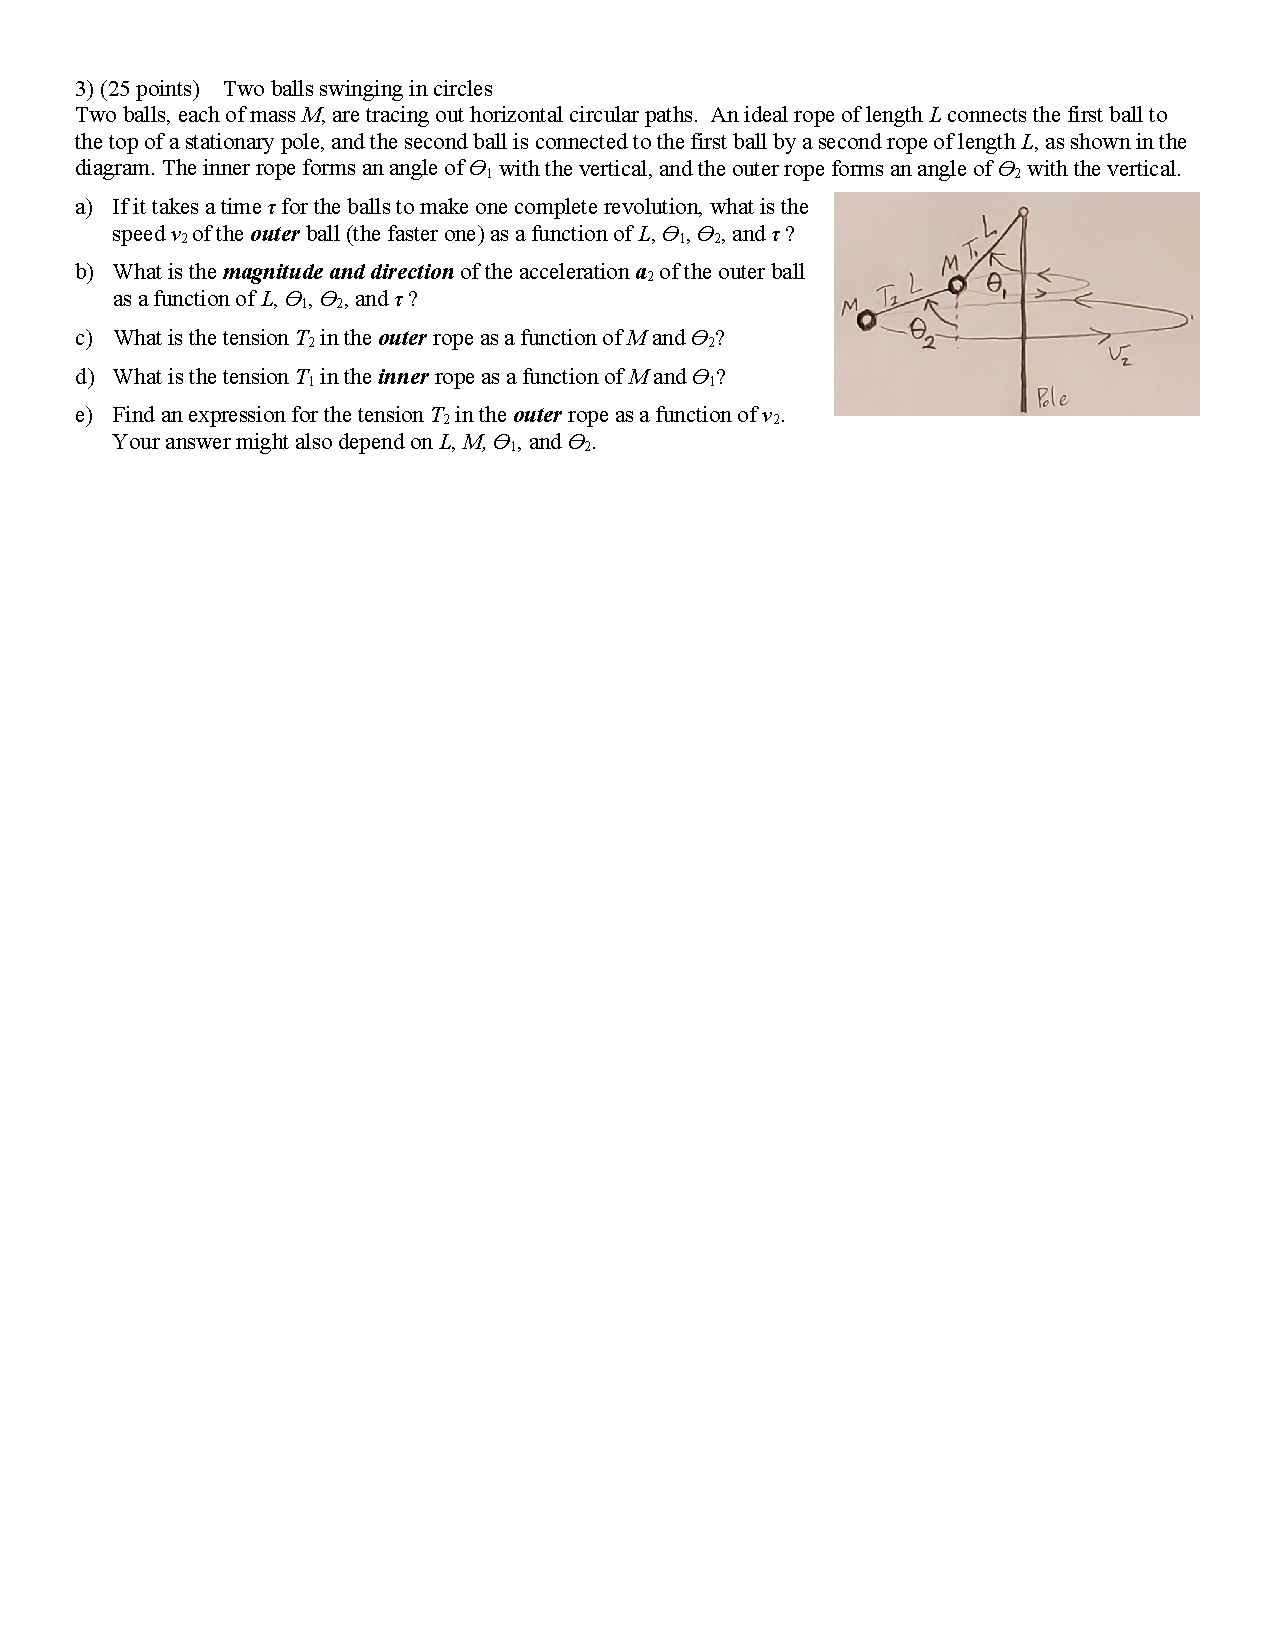
\includepdf[pages=-]{figs/0702/f22.pdf}
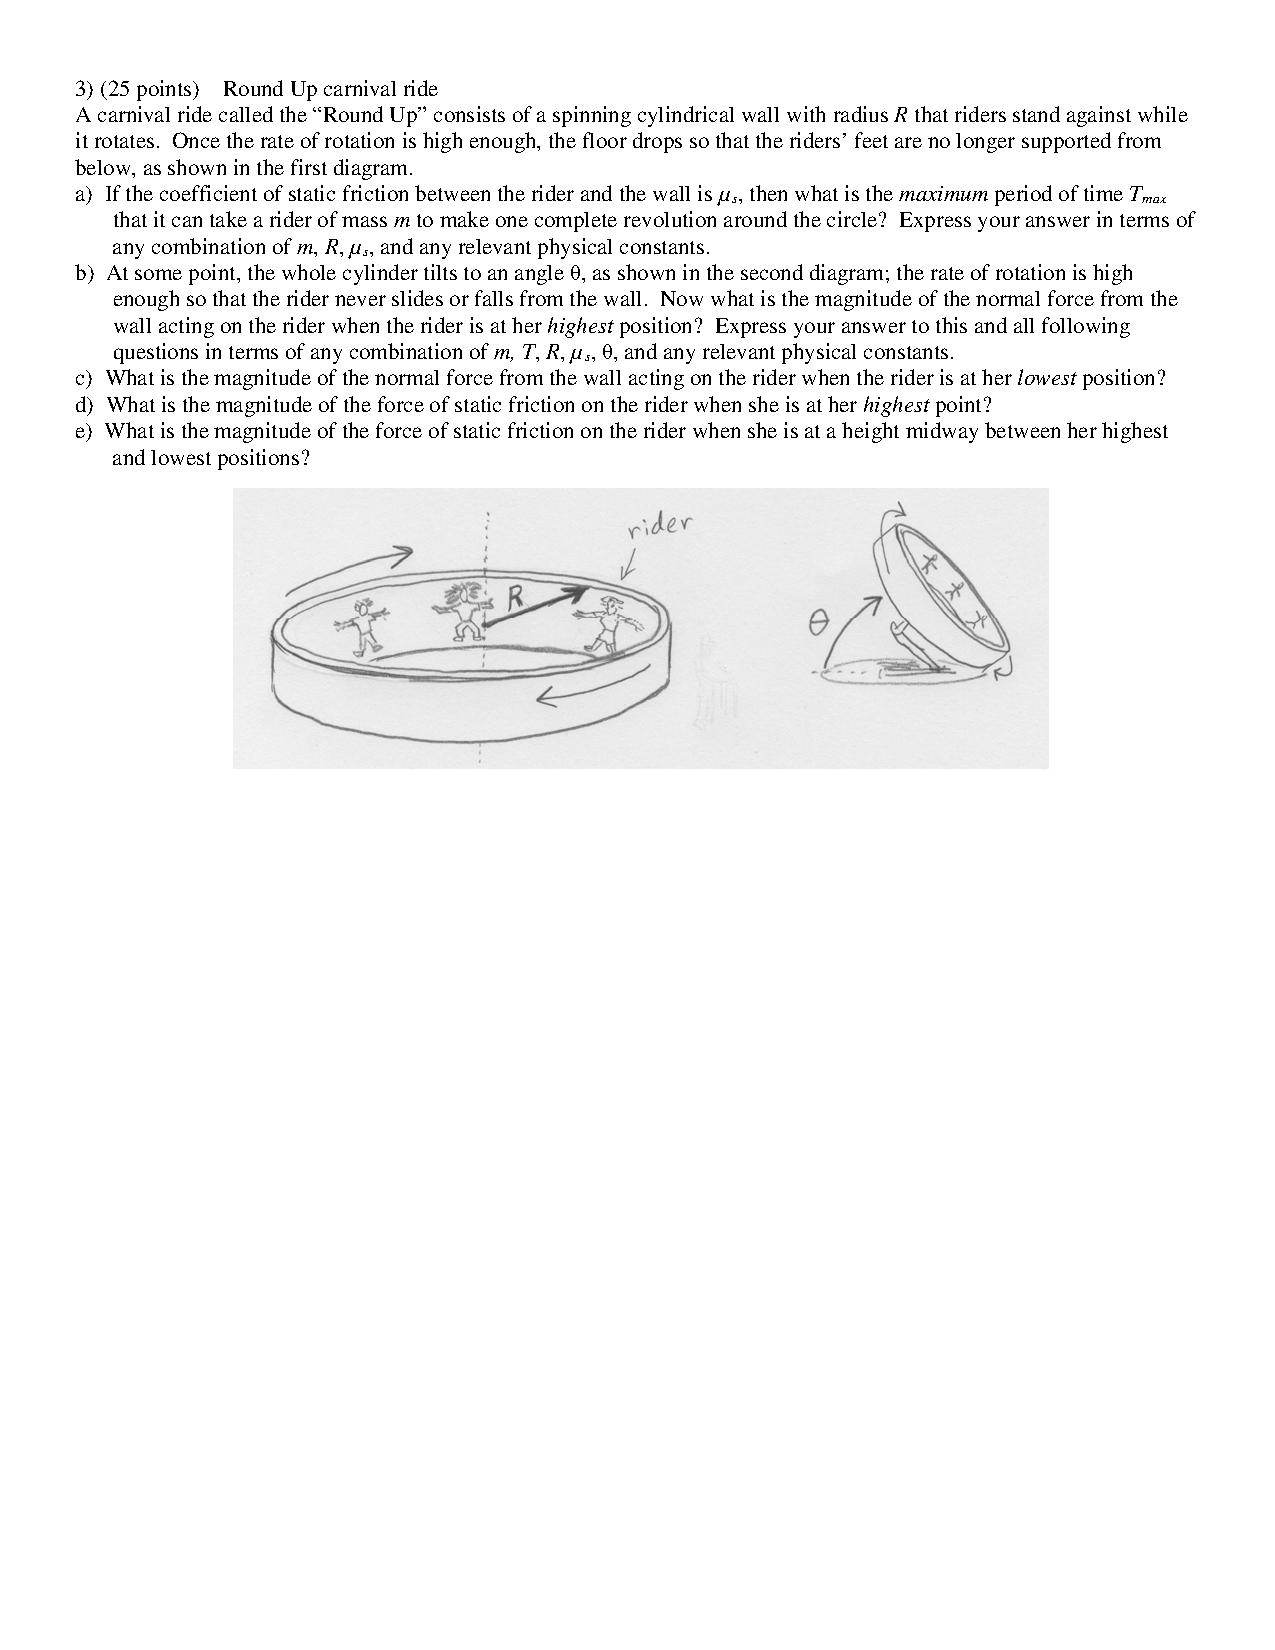
\includepdf[pages=-]{figs/0702/s16.pdf}
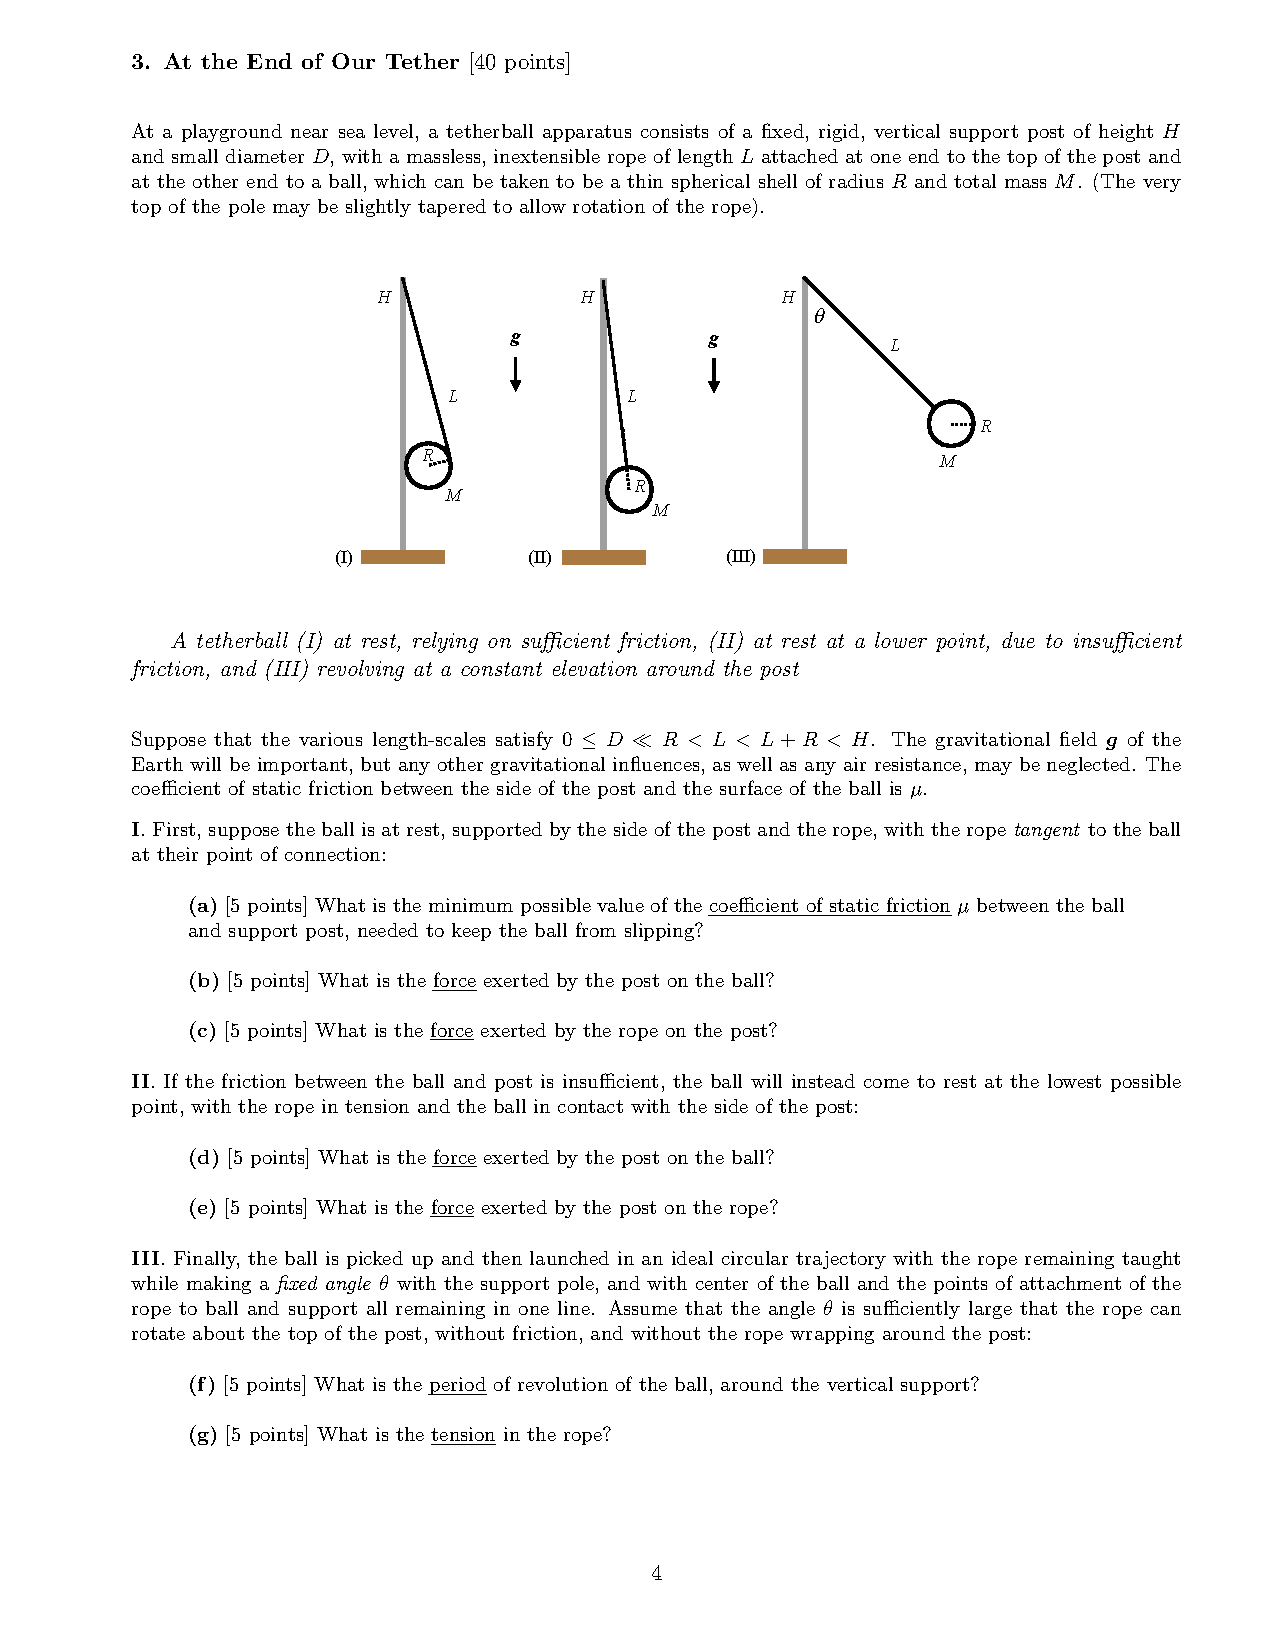
\includepdf[pages=-]{figs/0702/charman.pdf}

\end{document}
